% Presentation: Introduction to MOM
%     Location: CoE CMS Winter School, 12 July 2012
%       Author: Marshall Ward
%-----------------------------------------------------------------------------%
\documentclass[red]{beamer}

% Font configuration
\usepackage{pxfonts}

% Packages
\usepackage{listings}
\usepackage{hyperref}
\usepackage[squaren]{SIunits}

\usepackage{color}
\definecolor{ltblue}{rgb}{0.9, 0.9, 1.0}
\definecolor{dkgreen}{rgb}{0,0.6,0}
\definecolor{gray}{rgb}{0.5,0.5,0.5}
\definecolor{mauve}{rgb}{0.58,0,0.82}

% Beamer configuration
\usetheme{Frankfurt}

% LaTeX configuration
\graphicspath{{figures/}}

%=============================================================================%
\title{An Introduction to MOM}
\date{12 July 2012}

%=============================================================================%
\begin{document}
% Listings settings
\lstset{
    language=bash,
    basicstyle=\ttfamily,
    showspaces=false,
    showstringspaces=false,
    backgroundcolor=\color{ltblue},
    numberstyle=\tiny\color{gray},
    keywordstyle=\color{blue},
    commentstyle=\color{dkgreen},
    stringstyle=\color{mauve}
}

%-----------------------------------------------------------------------------%
\begin{frame}
    \titlepage
\end{frame}

%=============================================================================%
\section[Overview]{MOM4 Overview}

%-----------------------------------------------------------------------------%
\begin{frame}
    \frametitle{MOM4 Dynamic Core}
    
    \begin{itemize}
        \item Hydrostatic, Boussinesq
        \item Orthogonal Horizontal Grids
        \item Generalised vertical grids: $z, p$
		\item Explicit free surface
		\item Modern thermodynamic support
        \item Partial grid topograpy
    \end{itemize}
\end{frame}    

%-----------------------------------------------------------------------------%
\begin{frame}
    \frametitle{Orthogonal Horizontal Grids}
    
    \begin{center}
        \includegraphics<1>[width=0.7\textwidth]{merc_tripolar.pdf}
        \includegraphics<2>[width=0.5\textwidth]{nh_tripolar.pdf}
        \includegraphics<2>[width=0.5\textwidth]{sh_tripolar.pdf}
        \includegraphics<3>[width=0.7\textwidth]{merc_auscom.pdf}
    \end{center}
\end{frame}

%-----------------------------------------------------------------------------%
\begin{frame}
    \frametitle{Generalised Vertical Grids}
    
    \begin{itemize}
        \item Depth coordinates $z$ (Boussinesq)
         
        \item Hydrostatic pressure coordinates $p$ (Non-Boussinesq)
        
        \item Quasi-horizontal vertical grids:
            $z^* = H(\mathbf{x}) \left(\frac{z - \eta}{H + \eta}\right)$
        
        \item Limited support for terrain-following ($\sigma$) coordinates
    \end{itemize}
\end{frame}

%-----------------------------------------------------------------------------%
\begin{frame}
    \frametitle{Quasi-horizontal Vertical Grids}
    
    \begin{center}
        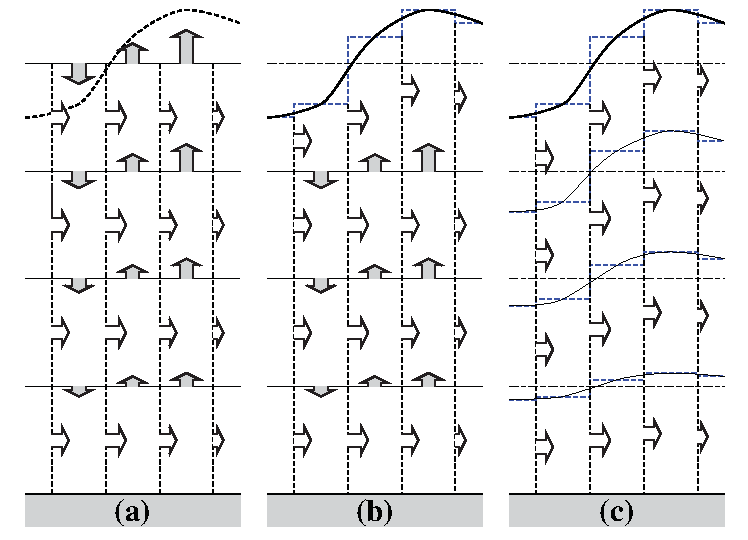
\includegraphics[width=0.8\textwidth]{zstar.pdf}
    \end{center}
    
    {\tiny "NEMO Ocean Engine", Madec et al. (2012)}
\end{frame}

%=============================================================================%
\section{MOM4 Quick User's guide}
%-----------------------------------------------------------------------------%
\begin{frame}
    \frametitle{Constructing a MOM4 Experiment}

    \begin{itemize}
        \item Acquiring the source code
        \item Creating a model grid
        \item Model configuration
        \item Compiling and running the model
    \end{itemize}

\end{frame}

%-----------------------------------------------------------------------------%
\begin{frame}[fragile]
    \frametitle{Acquiring the source code}
    
    Up-to-date versions of the source code are available on a subversion (svn)
    server hosted by NCI:
  
    \begin{lstlisting}
# Enter as one line
svn co https://access-svn.nci.org.au/mom4
               /branches/local_changes
    \end{lstlisting}
    Contact NCI for access (IP address required)
    
    \begin{itemize}
        \item \lstinline|mom4/trunk|: GFDL code release mirror
        \item \lstinline|local_changes|: Stable release on vayu
        \item \lstinline|future_local_changes|: Experimental release on vayu
    \end{itemize}
    
    \textit{Note: Expect changes to this in the future}
\end{frame}

%-----------------------------------------------------------------------------%
\begin{frame}
    \frametitle{Creating a model grid}
    
    Ocean-only (or \textit{solo}) simulations require the following:
    \begin{itemize}
        \item Vertical grid
        \item Horizontal grid
        \item Topography
        \item Mosaic manifest file
    \end{itemize}
\end{frame}
%-----------------------------------------------------------------------------%
\begin{frame}[fragile]
    \frametitle{Vertical Grid Generation}

    From your source code directory:
    \begin{lstlisting}
> cd src/tools/ocean_vgrid
> make
> # Uniform grid:
> ./ocean_vgrid --nbnds 2 --bnds 0,4000 --nz 40
> # Two-scale grid:
> ./ocean_vgrid --nbnds 3 --bnds 0,300,4000 --nz 20,20
    \end{lstlisting}

    Output is \textit{supergrid} (edges + faces)
    
    $N$ cells = $2N + 1$ grid points

    

\end{frame}

%=============================================================================%
\end{document}
